\documentclass[a4paper]{article}
\usepackage[english]{babel}
\usepackage[utf8]{inputenc}
\usepackage[margin=1.15in]{geometry}
\usepackage{amsmath}
\usepackage{setspace}
\usepackage[colorinlistoftodos]{todonotes}
\usepackage{verbatim}
\usepackage{graphicx}
\usepackage[export]{adjustbox}
\setlength{\parskip}{\baselineskip}
\setlength{\parindent}{0pt}


\usepackage{enumitem}

\title{QF603 Group Mini-Project 2}

\author{Group F}

\date{\today}

\begin{document}
	\maketitle
	
	\begin{abstract}
		In this report, we implemented a simple linear regression of the Dow Jones Industrial Average (“DJIA”) index over the S\&P500 (“S\&P”) using daily and annual log returns.
		 
		Our key finding is that the return characteristics of the DJIA does not exhibit statistically significant average excess returns as compared to the S\&P.
		 
		Another finding is that using different time intervals (daily vs annual log returns) to preform the regression leads to significant differences in the kurtosis measure of the distribution of the error terms in the regression. Investigating further, the reason for this difference is found to be due to the bias introduced into the annual data series when the last day of the year is used as a benchmark. We present further comparative illustrations to show this. 
		 	
	\end{abstract} 
	
	\newpage
	\setcounter{secnumdepth}{1}
	\section*{Task 3: Regression of Daily Log Returns}
	\label{sec:introduction}
	
	\begin{figure}[htbp]
		\centering
		\begin{minipage}[t]{0.48\textwidth}
			\centering
			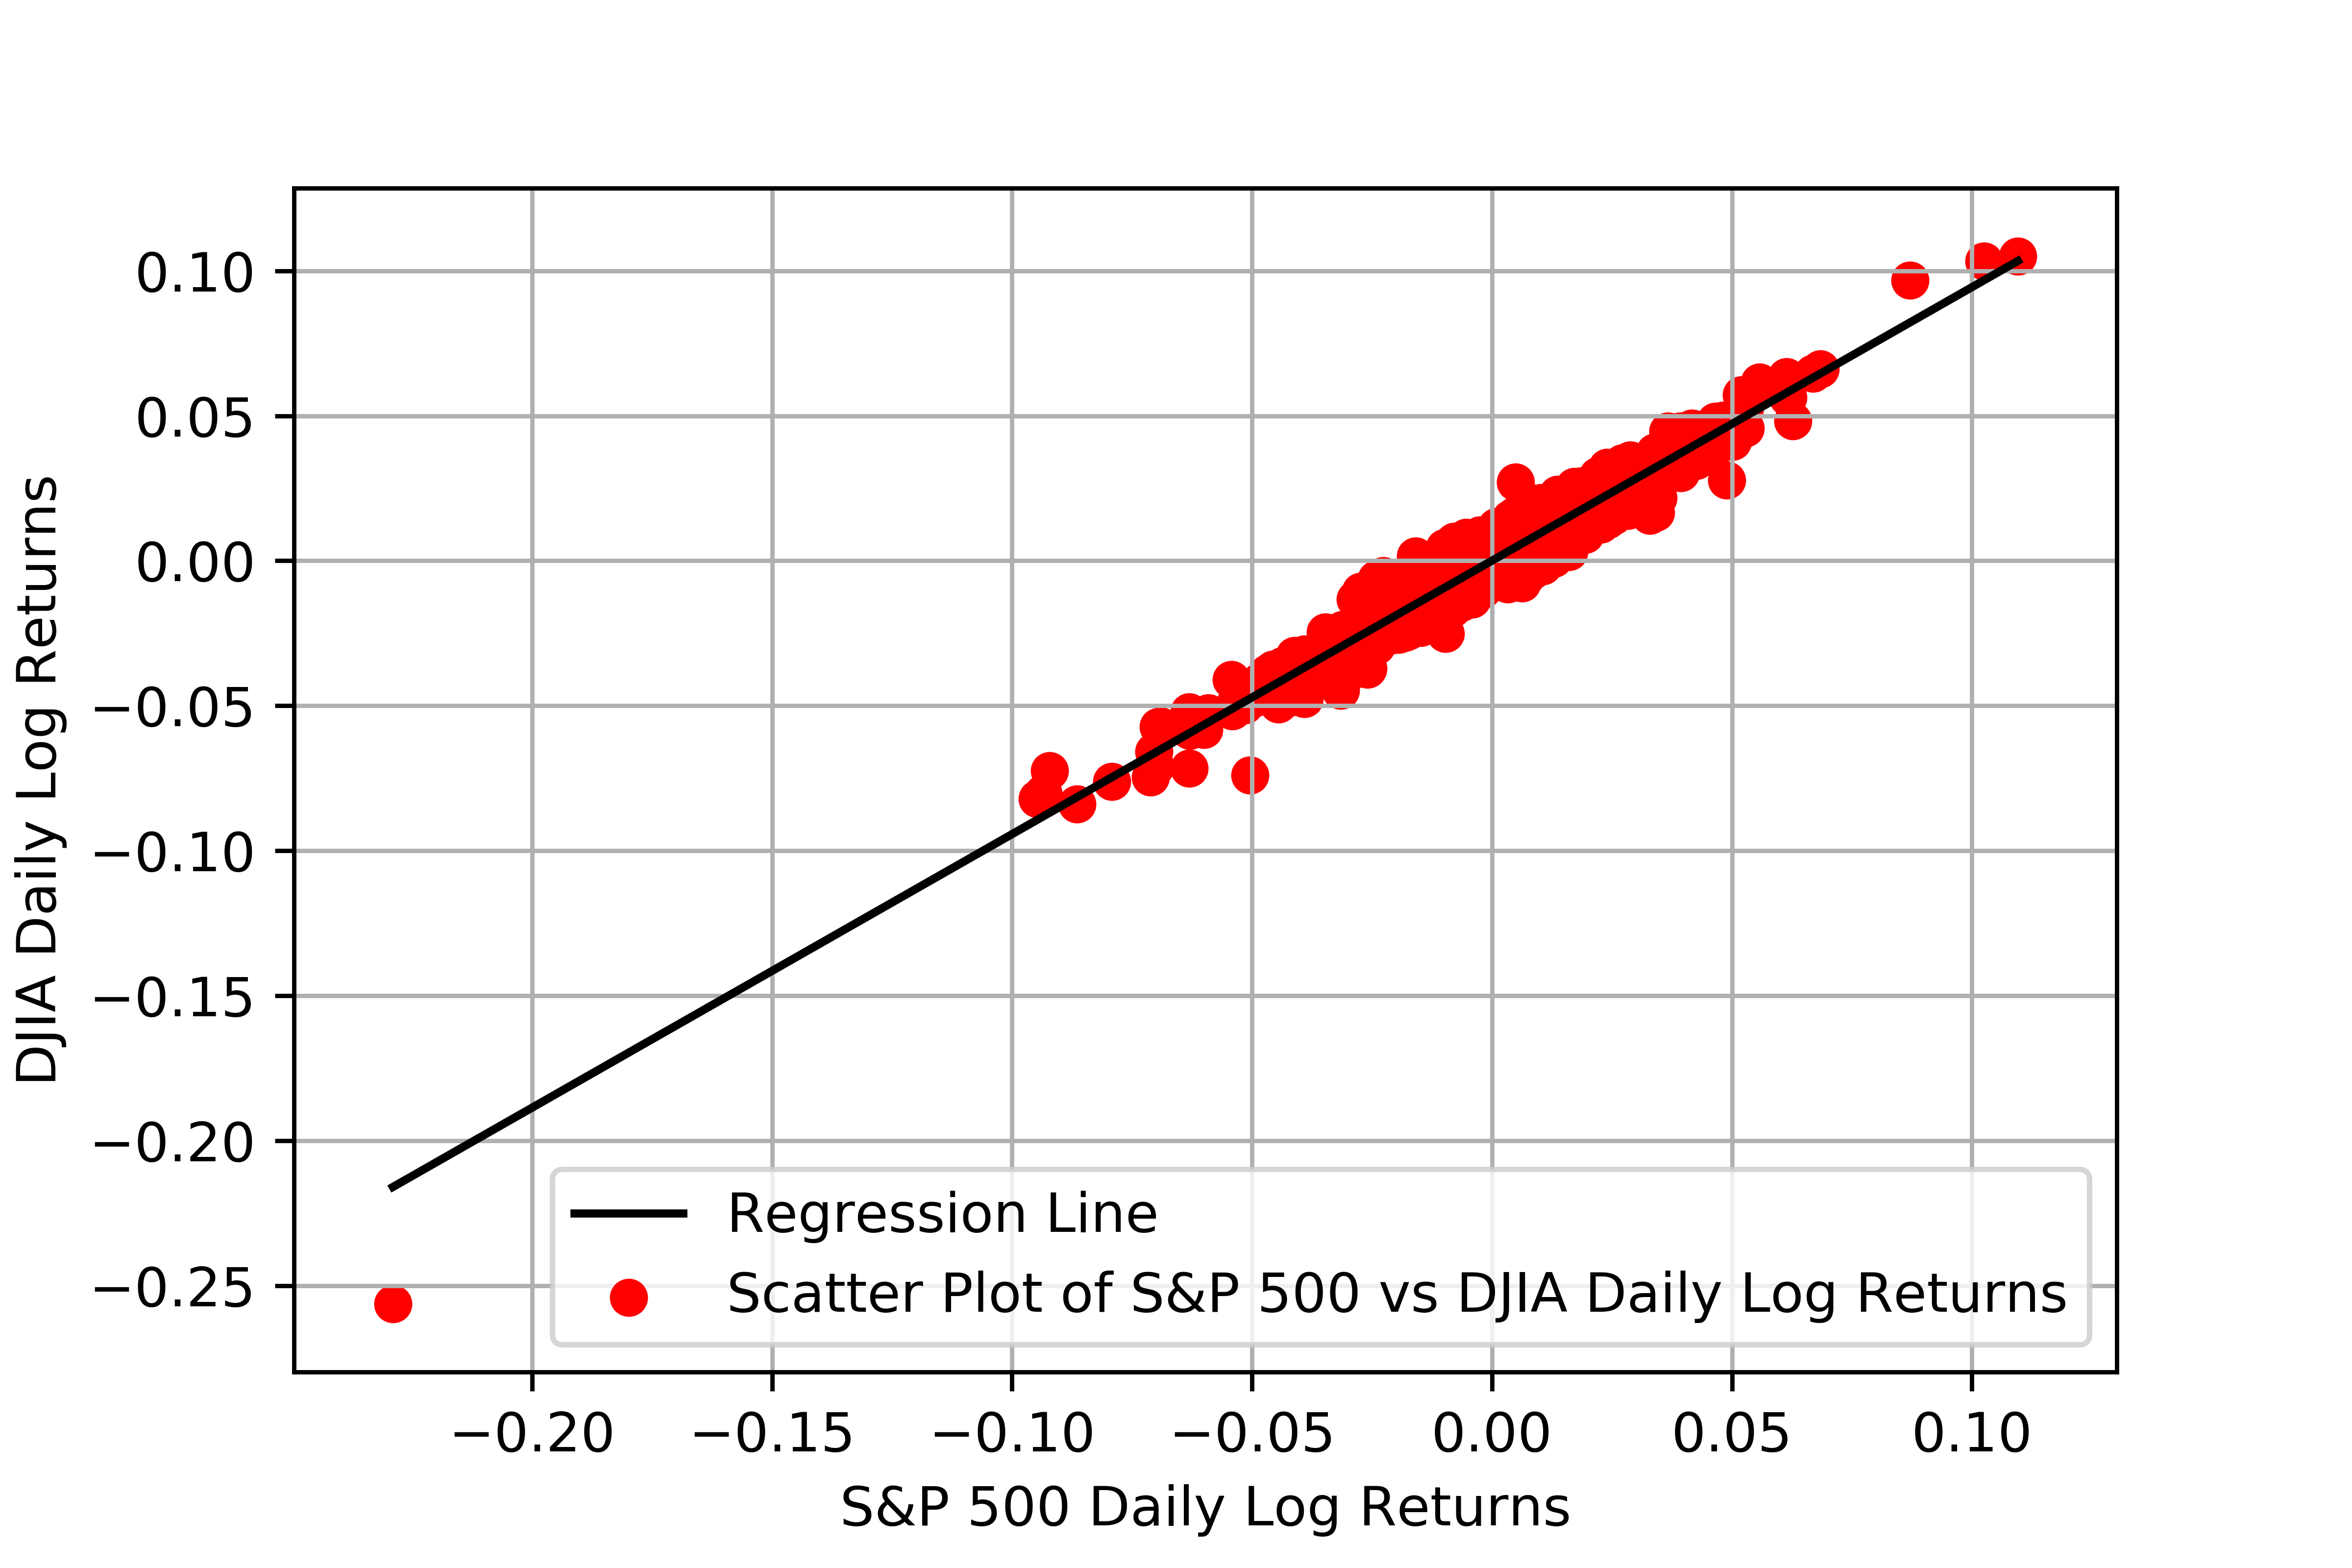
\includegraphics[width=6cm]{Daily_Scatter.png}
			\caption{Regression Line of Daily Log Return}
		\end{minipage}
		\begin{minipage}[t]{0.48\textwidth}
			\centering
			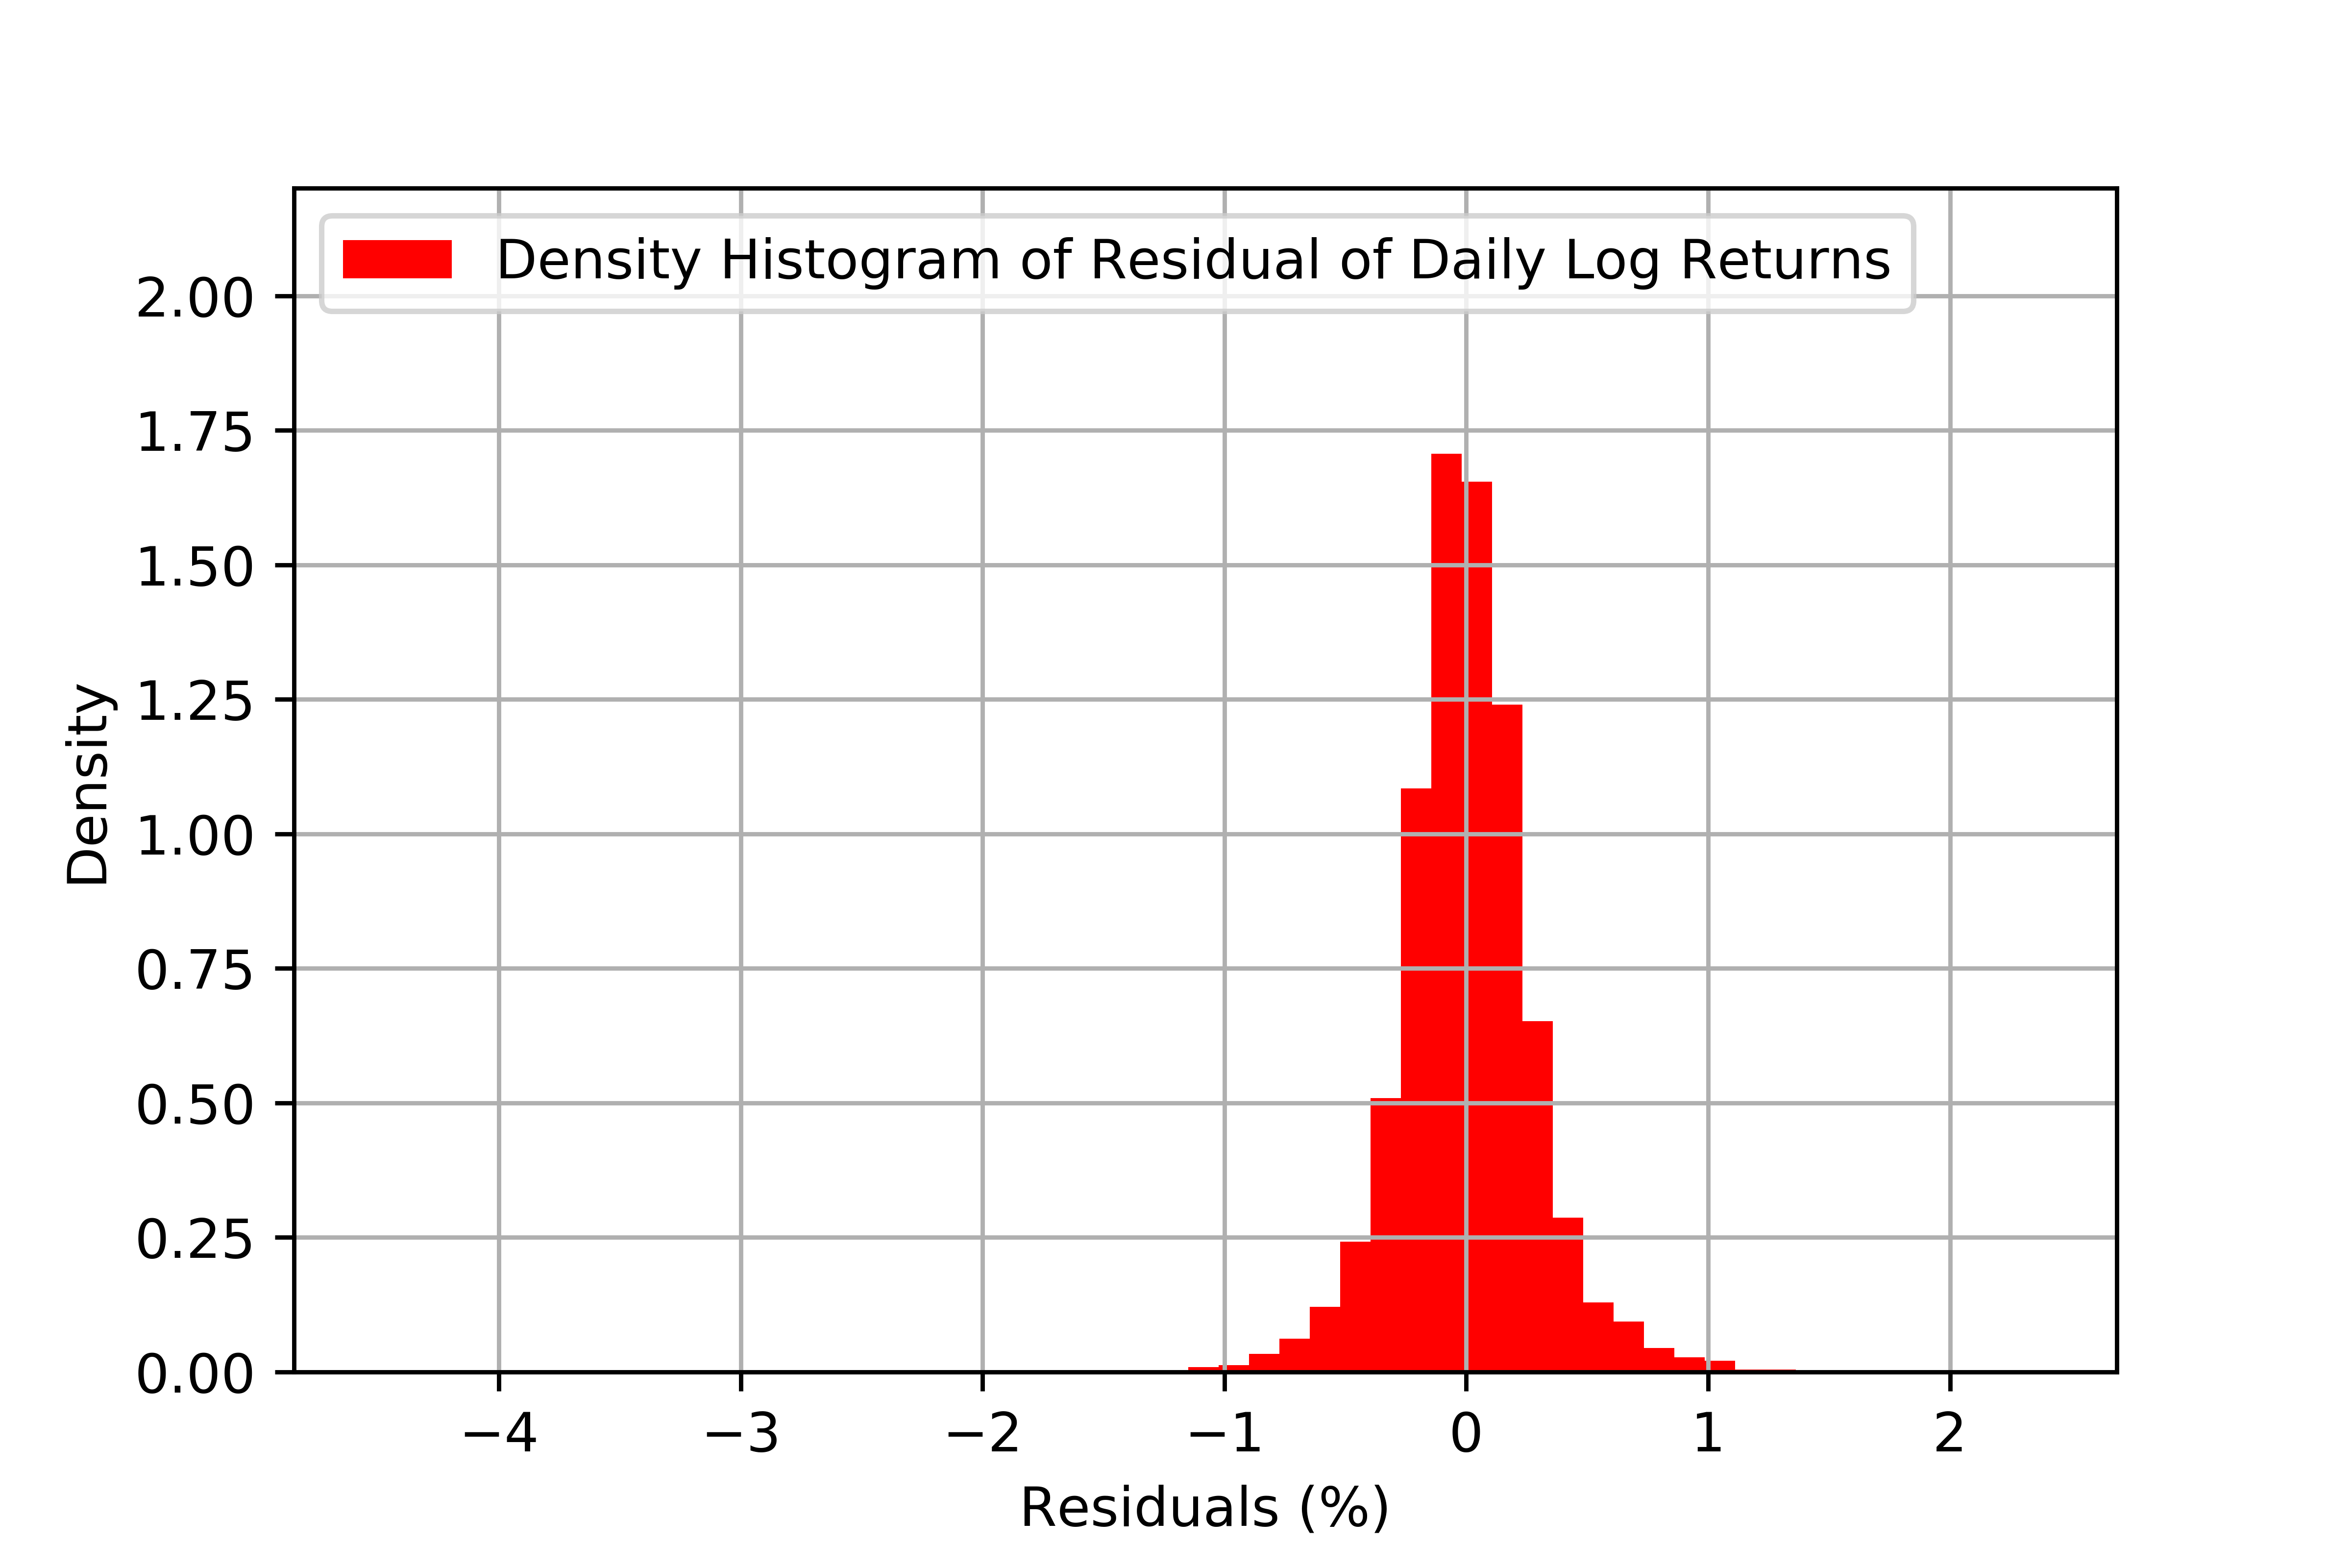
\includegraphics[width=6cm]{Daily_Hist.png}
<<<<<<< HEAD
			\caption{Density Histogram of Residuals from the Daily Log Return regression}
=======
			\caption{Desity Histogram of Residual}
>>>>>>> 4b5a1a4fded33820a1483528b97ebf7524a770f1
		\end{minipage}
	\end{figure}
	
	\subsection{Estimate of key statistics $\hat{a},\hat{b}$ and $\hat{\sigma}_{u_t}$}
	\underline{Results}
	\begin{itemize}[nosep]
		\item Alpha = $\hat{a} = -0.00005$, Beta = $\hat{b} = 0.94311$
		\item Standard Distribution of Residual = $\sigma_{u_t} = 0.00288$
	\end{itemize}

	The regression can be expressed as $r_{(DJIA, t)} = -0.00005 +  0.94311 r_{(S\&P500, t)}$.
	
	The positive intercept indicates that the DJIA has a small positive daily excess returns on average as compared to the S\&P. 
	
	The slope of 0.94311 indicates that the DJIA is slightly less volatile than the S\&P. In this context, the slope is interpreted as Beta – the sensitivity of DJIA’s returns to the S\&P’s returns. Assuming investors are risk-averse, a lower Beta is preferred for the same level of return because a lower Beta asset will have more consistency in its returns.
	  
	Combining these two measures together, it suggests that the DJIA has a superior risk-adjusted return as compared to the S\&P. 
	
	
	\subsection{T-test for Null Hypothesis a=b=0 at 5\% significance}
	\underline{Results}
	\begin{itemize}[nosep]
		\item T-statistics for $\hat{a} = 1.48636$, and for $\hat{b} = 339.97366$
		\item Degree of Freedom = $8500 - 2 = 8498$
		\item Null Hypotheses ($H_0$) are that $a=b=0$.
		\item Alternative hypotheses ($H_1$) are that $a\ne 0 \quad \textnormal{and} \quad b\ne 0$
		\item Critical value at 5\% significance level = $\pm1.96024$
	\end{itemize}
	
	\begin{comment}
	For $\hat{a}$, the test statistic lies within the 95\% confidence interval (i.e. does not exceed the 5\% critical level). Therefore, we do not reject the null hypothesis. The intercept coefficient $\hat{a}$ is not significantly different from 0 at the 5\% significance level.
	
	In contrast, for $\hat{b}$, the test statistic lies well beyond the 95\% confidence interval (i.e. significantly exceeds the 5\% critical level). Therefore, we reject the null hypothesis and accept the alternative hypothesis. The slope coefficient $\hat{b}$ is significantly different from 0 at the 5\% significance level.
	\end{comment}
	
	The test statistic for $\hat{a}$ falls within the critical values, and thus we cannot reject the null hypothesis that $\hat{a}=0$. The indication of DJIA having higher daily returns than the S\&P is therefore not significant at the 5\% level.  
	
	However, the test statistic for $\hat{b}$ falls outside the critical values, and thus we reject the null hypothesis that $\hat{b}=0$ and conclude that there is a linear relationship between DJIA and S\&P at the 5\% significance level. 
	
	
	\subsection{Goodness of Fit: $R^2$ and Adjusted $R^2$ values}
	\underline{Results}
	\begin{itemize}[nosep]
		\item R-Squared $(R^2) = 93.15120\%$
		\item Adjusted R-Squared $(\textnormal{adj-}R^2) = 93.1539\%$
	\end{itemize}
	\begin{comment}
	The $R^2$ value is very high, further supporting our previous point that there exists a linear relationship between the daily returns of the DJIA and the S\&P.
	\end{comment}

	The $R^2$ value reports the degree to which our independent variable (the SP500 daily log returns) explains the variation of the dependent variable (the DJIA daily log returns). Since R-square is 93.15120\%, it means that over 90\% of the variation in the dependent variable is explained by the independent variable.
	
	$\textnormal{Adj-}R^2$ also measures the goodness of model fitting, but takes into consideration the number of independent variables in the model. $R^2$ will only increase or  stay the same when we add more independent variables, even if they do not have any relationship with the dependent variable. $\textnormal{Adj-}R^2$ on the other hand, will "penalize" the model for having excessive dependent variables that do not significantly improve the model. 
	
	The $\textnormal{adj-}R^2$ is always lower than the $R^2$ value. And, in our case, because there is only 1 independent variable, the $\textnormal{adj-}R^2$ and the $R^2$ values are relatively equal.
	
	\subsection{Jarque-Bera test statistic for the residuals}
	\underline{Results}
	\begin{itemize}[nosep]
		\item Jarque-Bera test stats = 25434.27
		\item Degrees of Freedom = 2
		\item Null Hypothesis $H_0 = 0$
		\item Alternative Hypothesis $H_1 \ne 0$
		\item Critical Chi-Square Value at 5\% significance level = 5.99146
	\end{itemize}
	
	The JB test statistic exceeds the critical value by a huge margin, strongly indicating that the residuals are not normally distributed. This is due to regression outliers that were a result of extreme market conditions, for example the huge one-day drop on 19-Oct-1987. 
	
	\begin{comment}
	The JB test's null hypothesis is JB = 0. If the null hypothesis is not rejected, it indicates that the
	distribution of the errors are normally distributed (under a certain level of significance).
	\end{comment}

	\subsection{Additional test-$H_0$: $\hat{b}=1$}
	\underline{Results}
	\begin{itemize}[nosep]
		\item The t-test statistic for $\hat{b}=1$=-20.50787
		\item Degree of Freedom= $8500 - 2 = 8498$
		\item Null Hypothesis ($H_0$) is that $\hat{b}=1$
		\item Alternative hypothesis ($H_1$) is that $\hat{b} \ne 1$
		\item Critical value at 5\% significance level = $\pm 1.96024$
	\end{itemize}

	We conduct an additional test of $\hat{b}=1$ at the 5\% significance level to determine if our $\hat{b}$ value of 0.94311 is statistically different from 1. We do this to gauge how well the returns of the DJIA mimic the returns of the market portfolio S\&P.
	
	We reject the null hypothesis that $\hat{b}=1$, and conclude that the daily log returns of the DJIA do not perfectly mimic the returns of the S\&P. Therefore, using the DJIA as a benchmark for performance evaluation may lead to different results as compared to when using the S\&P as the benchmark. 
		
	\section*{Task 4: Regression of Yearly Log Returns}
	\label{sec:num2}
	
	\begin{figure}[htbp]
		\centering
		\begin{minipage}[t]{0.48\textwidth}
			\centering
			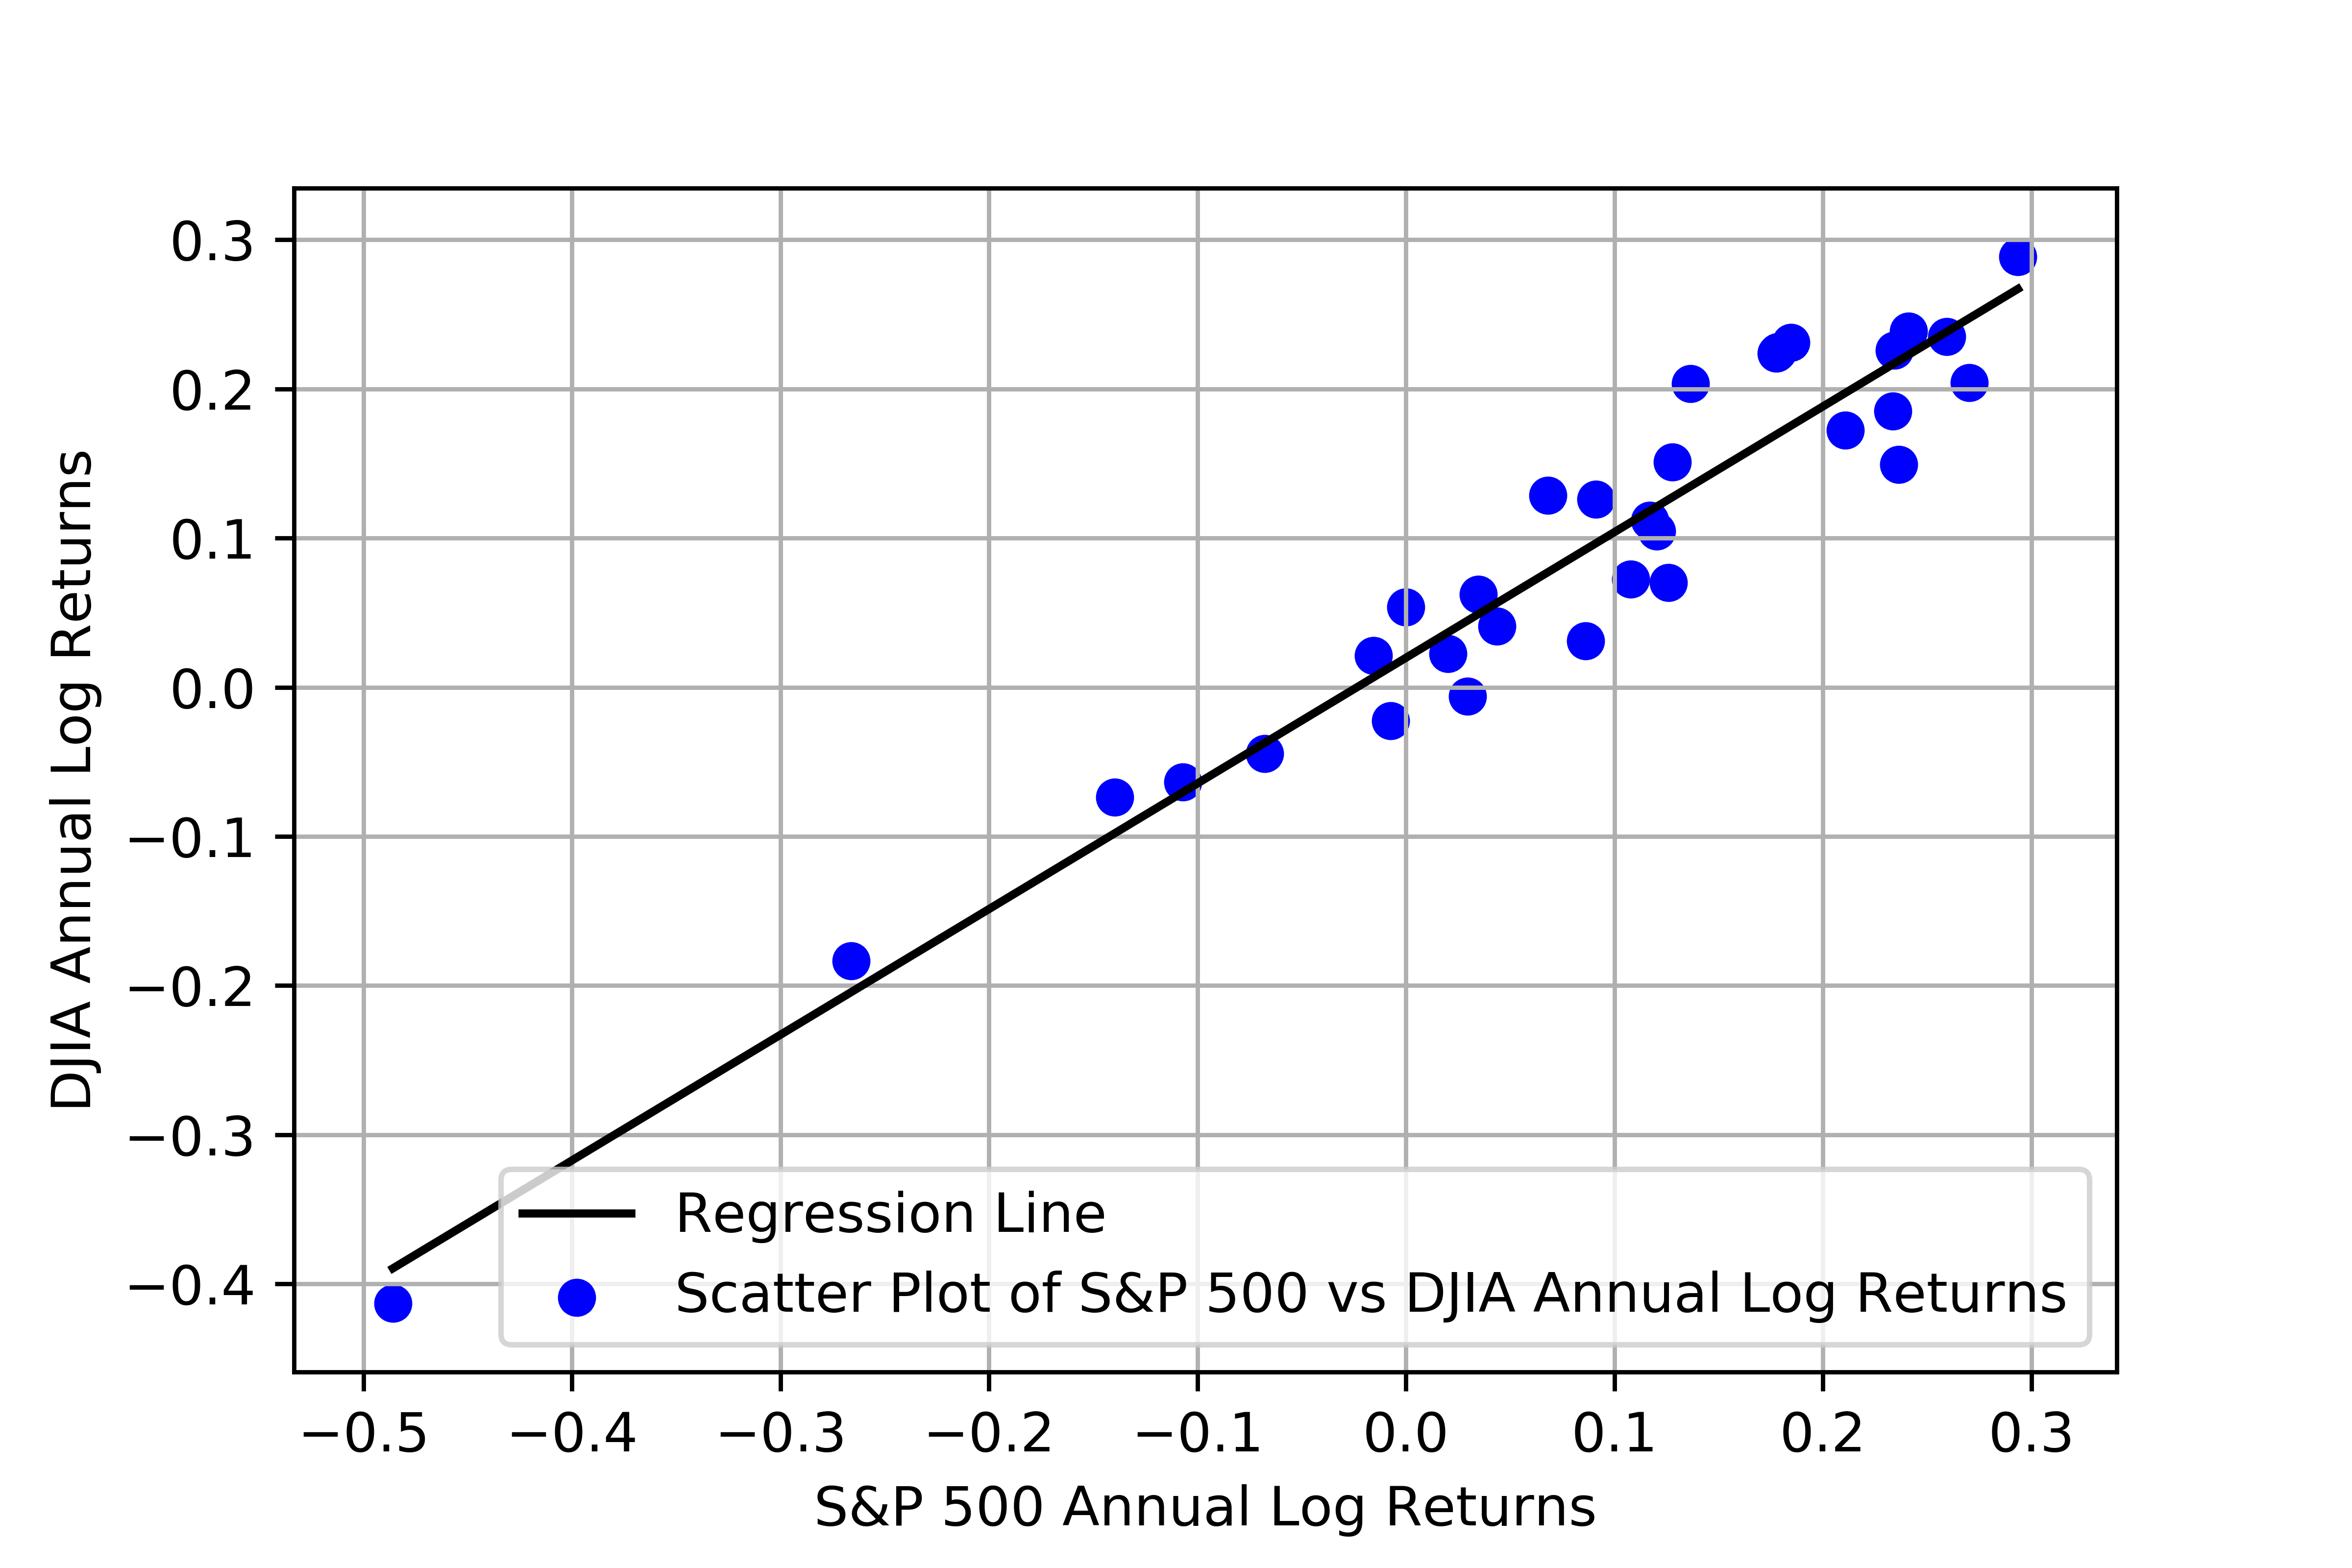
\includegraphics[width=6cm]{Ann_Scatter.png}
			\caption{Regression Line of Annual Log Return}
		\end{minipage}
		\begin{minipage}[t]{0.48\textwidth}
			\centering
			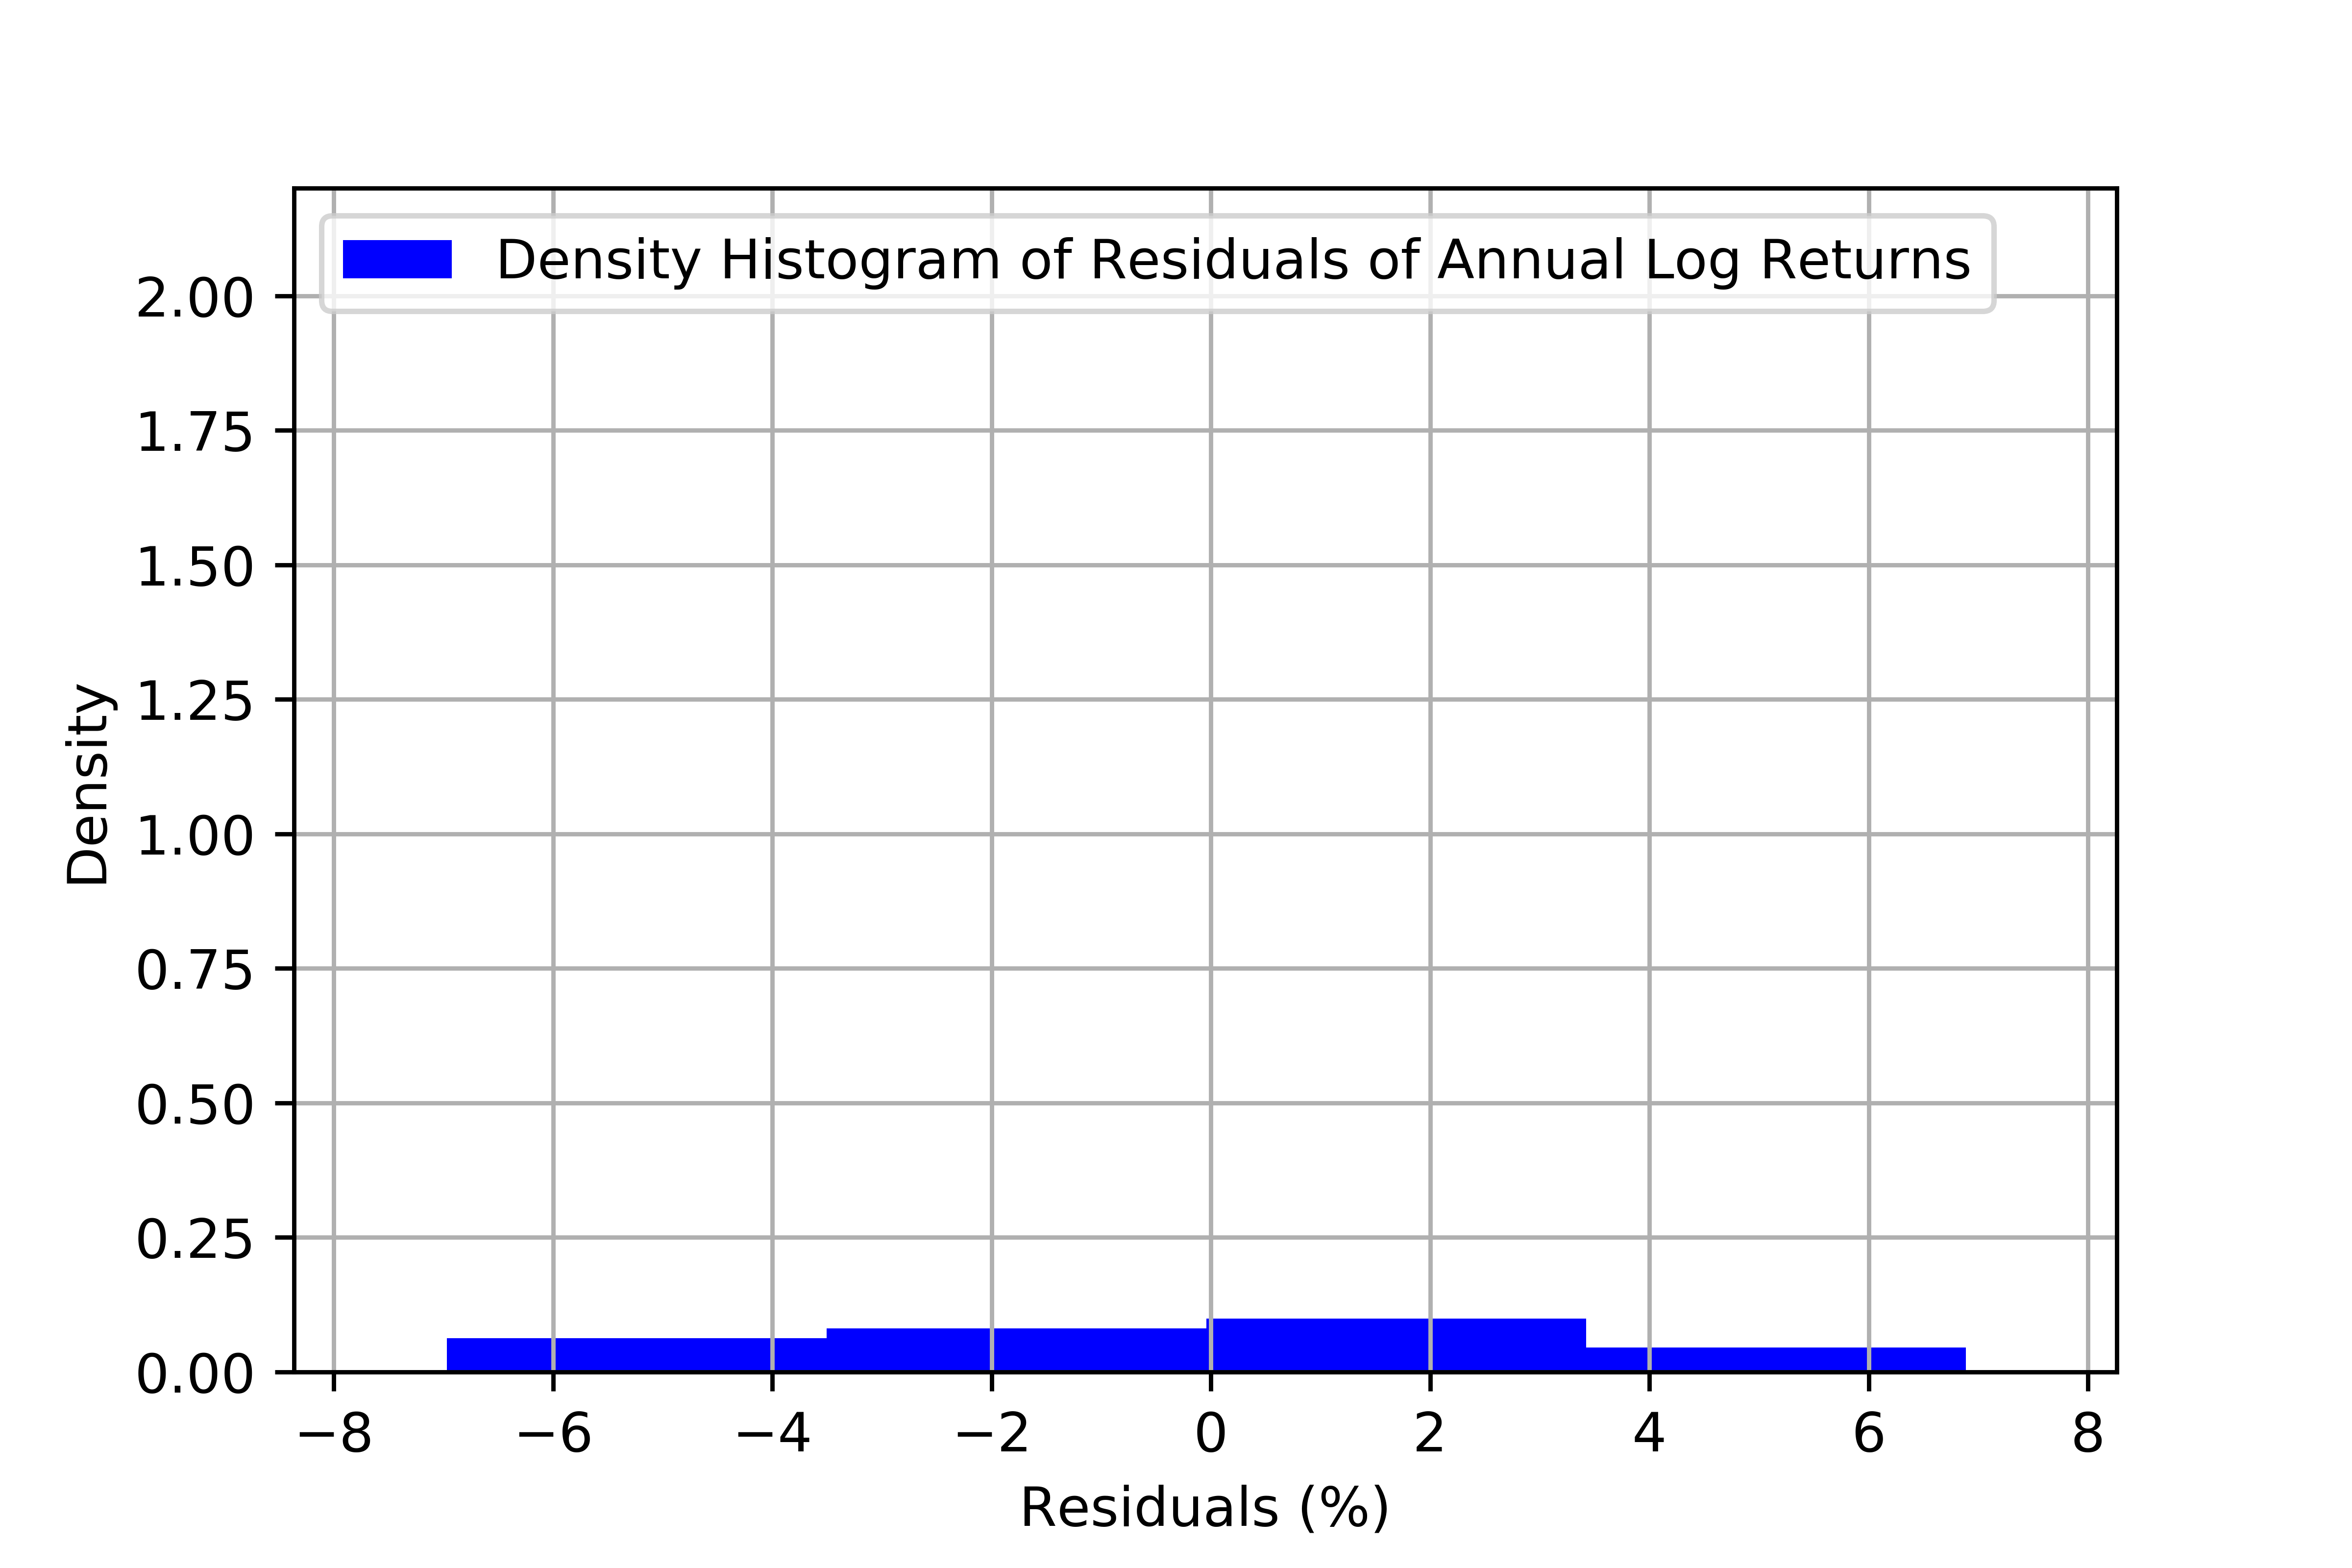
\includegraphics[width=6cm]{Ann_Hist.png}
<<<<<<< HEAD
			\caption{Density Histogram of Residuals from the Annual Log Return regression}
=======
			\caption{Density Histogram of Residual}
>>>>>>> 4b5a1a4fded33820a1483528b97ebf7524a770f1
		\end{minipage}
	\end{figure}
	
	\subsection{Estimate of key statistics $\hat{a}$,$\hat{b}$ and $\hat{\sigma_u}$}
	\underline{Results}
	\begin{itemize}[nosep]
		\item Alpha = $\hat{a} = 0.01978$, Beta = $\hat{b} = 0.84254$
		\item Standard Distribution of Residual = $\sigma_{u_t} = 0.03797$
	\end{itemize}

    The regression can be expressed as $r_{(DJIA, t)} = 0.01978 +  0.84254 r_{(S\&P500, t)}$.
	
	The positive intercept indicates that the DJIA has a small positive daily excess returns on average as compared to the S\&P. 
	
	The slope of 0.8425 indicates that the DJIA is slightly less volatile than the S\&P. 
	
	Combining these two measures together, it suggests that the DJIA has a superior risk-adjusted return as compared to the S\&P. 
	
	
	\subsection{T-test for Null Hypothesis a=b=0 at 5\% significance}
	\underline{Results}
	\begin{itemize}[nosep]
		\item T-statistics for $\hat{a} = 2.64989$, and for $\hat{b} = 20.4364$
		\item Degree of Freedom = $32 - 2 = 30$
		\item Null Hypothesis ($H_0$) are that $a=b=0$.
		\item Alternative hypothesis ($H_1$) are that $a\ne 0 \quad \textnormal{and} \quad b\ne 0$
		\item Critical value at 5\% significance level = $\pm2.042272$
	\end{itemize}

    The test statistic for $\hat{a}$ falls outside the critical values, and thus we reject the null hypothesis that $\hat{a}$=0. The t-test at 5\% significance concludes that the DJIA has higher annual returns as compared to the S\&P.  
    
    The test statistic for $\hat{b}$ also falls outside the critical values, and thus we reject the null hypothesis that $\hat{b}$=0 and conclude that there is a linear relationship between the annual returns of the DJIA and the S\&P at the 5\% significance level.

	\subsection{Goodness of Fit: $R^2$ and Adjusted $R^2$ values}
	\underline{Results}
	\begin{itemize}[nosep]
		\item R-Squared $(R^2) = 0.932983$
		\item Adjusted R-Squared $(\textnormal{adj-}R^2) = 0.930749$
	\end{itemize}

     The $R^2$ value is very high, further supporting our previous point that there exists a linear relationship between the annual returns of the DJIA and the S\&P.
	
	\subsection{Jarque-Bera test statistic for the residuals}
	\underline{Results}
	\begin{itemize}[nosep]
		\item Jarque-Bera test stats = 25434.27
		\item Degrees of Freedom = 2
		\item Null Hypothesis $H_0 = 0$
		\item Alternative Hypothesis $H_1 \ne 0$
		\item Critical Chi-Square Value at 5\% significance level = 5.99146
	\end{itemize}
	
	The JB test statistic falls within the critical value, indicating that the regression residuals are normally distributed. We note that this finding is in contrast to the JB test performed for the daily log returns, and would like to investigate further as to the possible reason why this may be so.
	
	When we observe the density histograms (at the top of each section) we can see the stark difference in the distribution of the residuals. Although the histogram of residuals from the daily log returns regression has a more bell-like shape, that distribution fails the JB test. On closer inspection, we note that there are large negative outliers in the the histogram of residuals from the regression of the daily log returns (as can be seen from the range of the x-axis). We, therefore, suspect that it is these large outliers that caused the distribution to fail the JB test; by increasing the kurtosis of the distribution beyond what is tolerable under a normal distribution.
	
	When we plot the top 100 "worst days" (i.e. largest loss) log returns by month, we can see that most of the worse days do not even fall in December, let alone the 31st. Clearly, there is a greater number of outliers "included" in the daily return residuals. 
	
	\begin{figure}[ht]
		\centering
		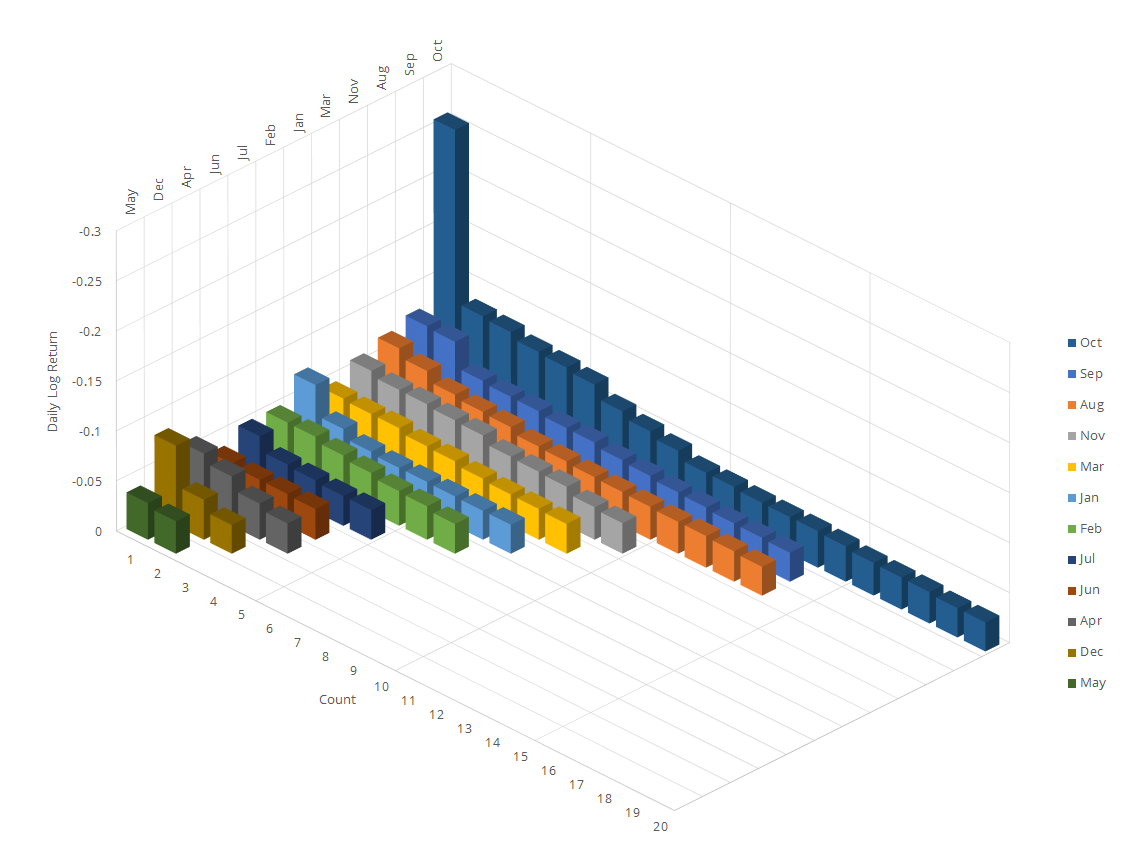
\includegraphics[width=0.6\linewidth, frame]{worstdays.png}
		\caption{Chart of Top 100 Largest Negative Log Returns}
	\end{figure}
	
	The exclusion of these outliers in the annual log return regression probably "saved" it from failing the JB test. 
	
	\subsection{Additional test-$H_0$: $\hat{b}=1$}
	\underline{Results}
	\begin{itemize}[nosep]
		\item The t-test statistic for $\hat{b}=1$=-3.81917
		\item Degree of Freedom=$32 - 2 = 30$
		\item Null Hypothesis ($H_0$) is that $\hat{b}=1$
		\item Alternative hypothesis ($H_1$) is that $\hat{b} \ne 1$
		\item Critical value at 5\% significance level = $\pm 1.96024$
	\end{itemize}
	
	We conduct an additional test of $\hat{b}=1$ at the 5\% significance level to determine if our $\hat{b}=1$ value of 0.84254 is statistically different from 1. We do this to gauge how well the returns of the DJIA mimic the returns of the market portfolio S\&P. 
	
	We reject the null hypothesis that $\hat{b}=1$, and conclude that the annual log returns of the DJIA do not perfectly mimic the returns of the S\&P. Therefore, using the DJIA as a benchmark for performance evaluation may lead to different results as compared to when using the S\&P as the benchmark. 
	
\end{document}
